\documentclass[11pt]{article}

% ---------------------------------------------------------------------------
% Packages
% ---------------------------------------------------------------------------
\usepackage[a4paper,margin=2.3cm]{geometry}
\usepackage{amsmath,amssymb}
\usepackage{booktabs}
\usepackage{array}
\usepackage{xcolor}
\usepackage{tikz}
\usepackage{enumitem}
\usepackage{hyperref}
\usetikzlibrary{arrows.meta,positioning,calc,shapes.geometric,decorations.pathreplacing}

\definecolor{navyblue}{RGB}{15,60,110}
\definecolor{seagreen}{RGB}{20,120,90}
\definecolor{softgray}{RGB}{120,120,120}
\definecolor{lightblue}{RGB}{225,238,250}
\definecolor{lightgreen}{RGB}{225,245,235}
\definecolor{lightgray}{RGB}{238,238,238}

\hypersetup{colorlinks=true,linkcolor=navyblue,urlcolor=navyblue}

\newcommand{\good}{\textcolor{seagreen}{\textbf{Yes}}}
\newcommand{\bad}{\textcolor{red!70!black}{\textbf{No}}}
\newcommand{\partly}{\textcolor{orange!80!black}{\textbf{Partial}}}

\title{\vspace{-1.5em}\textbf{\color{navyblue} Selecting a Motion Model for Autonomous Maritime\\ Vessel Testing in esmini / Unreal Engine}}
\author{Marine ASV Simulation --- Method Justification}
\date{\today}

% ---------------------------------------------------------------------------
\begin{document}
\maketitle
\vspace{-1.5em}

% ===========================================================================
\section{Problem Statement}
% ===========================================================================
The first prototype drove the vessel using a \textbf{Streaming Rigid Position Trajectory (SRPT)}:
a pre-computed list of $(x,y)$ positions replayed frame-by-frame. This is unsuitable for testing
an autonomous vessel, because the boat's motion is \emph{scripted in advance} and cannot
\emph{react}. My supervisor asked me to research a better approach. Three candidates were
considered:

\begin{enumerate}[leftmargin=1.6em]
    \item \textbf{Physics-driven closed-loop guidance} (start point $\rightarrow$ waypoints $\rightarrow$ end point). \textit{(chosen)}
    \item \textbf{Point-to-point physics} (steer straight from start to end, no path-following law).
    \item \textbf{Reusing car tracks as marine lanes} (drive the boat along OpenDRIVE lanes like a road vehicle).
\end{enumerate}

This document explains the chosen method at a high level, compares all four options, and shows
why the chosen method is the only one capable of validating the full COLREGs movement scenario
catalogue.

% ===========================================================================
\section{The Chosen Method (High Level)}
% ===========================================================================
The vessel is driven by a \textbf{Guidance--Navigation--Control (GNC)} architecture --- the same
structure used in real autonomous surface vessels. Motion is not scripted; it \emph{emerges} from
forces acting on a physical vessel model, corrected continuously by feedback.

\begin{center}
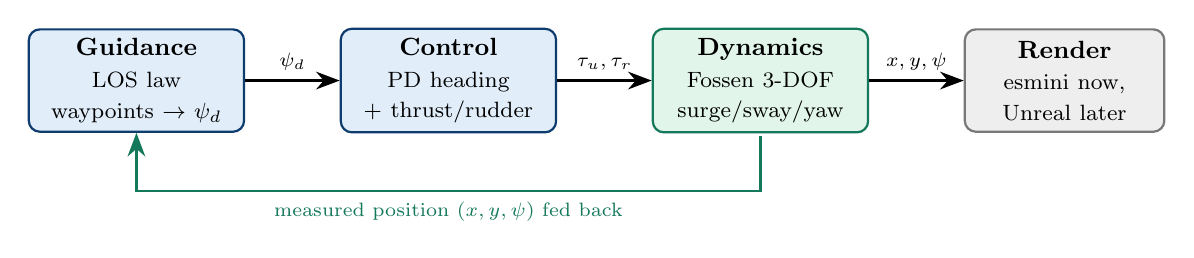
\begin{tikzpicture}[
    node distance=8mm and 12mm,
    block/.style={rectangle, rounded corners, draw=navyblue, thick,
        fill=lightblue, minimum height=13mm, text width=25mm, align=center, font=\small},
    plant/.style={rectangle, rounded corners, draw=seagreen, thick,
        fill=lightgreen, minimum height=13mm, text width=25mm, align=center, font=\small},
    sink/.style={rectangle, rounded corners, draw=softgray, thick,
        fill=lightgray, minimum height=13mm, text width=23mm, align=center, font=\small},
    arr/.style={-{Stealth[length=3mm]}, thick}
]
\node[block] (guid) {\textbf{Guidance}\\[2pt]\footnotesize LOS law\\ waypoints $\rightarrow \psi_d$};
\node[block, right=of guid] (ctrl) {\textbf{Control}\\[2pt]\footnotesize PD heading\\ + thrust/rudder};
\node[plant, right=of ctrl] (dyn) {\textbf{Dynamics}\\[2pt]\footnotesize Fossen 3-DOF\\ surge/sway/yaw};
\node[sink, right=of dyn] (viz) {\textbf{Render}\\[2pt]\footnotesize esmini now,\\ Unreal later};

\draw[arr] (guid) -- node[above,font=\scriptsize]{$\psi_d$} (ctrl);
\draw[arr] (ctrl) -- node[above,font=\scriptsize]{$\tau_u,\tau_r$} (dyn);
\draw[arr] (dyn) -- node[above,font=\scriptsize]{$x,y,\psi$} (viz);

% feedback loop
\draw[arr, seagreen]
    ($(dyn.south)+(0,-1pt)$) -- ++(0,-7mm)
    -| node[below, pos=0.25, font=\scriptsize]{measured position $(x,y,\psi)$ fed back} (guid.south);
\end{tikzpicture}
\end{center}

\noindent\textbf{The three stages:}
\begin{itemize}[leftmargin=1.6em]
    \item \textbf{Guidance --- Line-of-Sight (LOS).} Given sparse waypoints, LOS computes the desired
    heading $\psi_d$ needed to converge onto the \emph{path line} between waypoints. It reacts to the
    vessel's real position, so drift (e.g.\ from current) is detected and corrected.
    \item \textbf{Control --- PD + proportional actuators.} A heading controller converts the heading
    error into a commanded yaw rate; thrust and rudder controllers turn commands into forces/torques.
    \item \textbf{Dynamics --- Fossen 3-DOF model.} Newton--Euler equations with mass, added mass,
    Coriolis/centripetal coupling, and hydrodynamic damping produce realistic momentum, turning
    circles, sideways drift (sway), and stopping distances.
\end{itemize}

\subsection*{Line-of-Sight geometry and cross-track error}
The key feedback signal is the \textbf{cross-track error} $e$: the perpendicular distance from the
vessel to the intended path. LOS steers to drive $e \rightarrow 0$.

\begin{center}
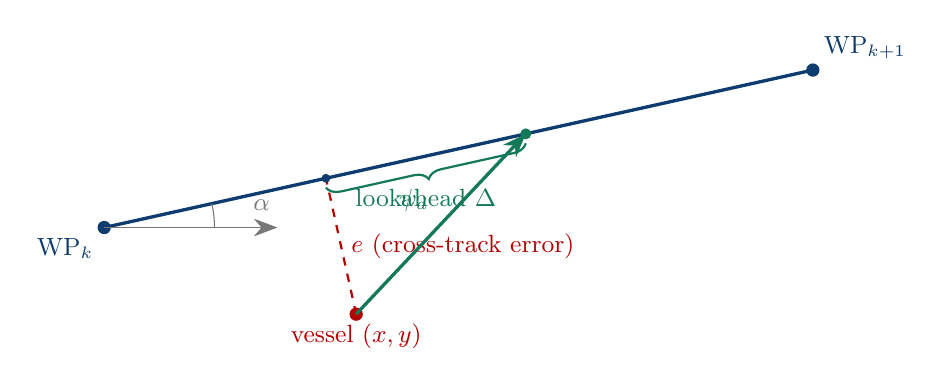
\begin{tikzpicture}[scale=1.0, >={Stealth[length=3mm]}]
% path line
\coordinate (wa) at (0,0);
\coordinate (wb) at (9,2);
\draw[navyblue, very thick] (wa) -- (wb)
    node[pos=0.0, below left, font=\small]{WP$_{k}$}
    node[pos=1.0, above right, font=\small]{WP$_{k+1}$};
\fill[navyblue] (wa) circle (2.4pt);
\fill[navyblue] (wb) circle (2.4pt);

% vessel position off the path
\coordinate (ship) at (3.2,-1.1);
\fill[red!70!black] (ship) circle (2.4pt);
\node[below, font=\small, red!70!black] at (ship) {vessel $(x,y)$};

% foot of perpendicular onto path
\coordinate (foot) at ($(wa)!(ship)!(wb)$);
\draw[red!70!black, thick, dashed] (ship) -- (foot)
    node[midway, right, font=\small]{$e$ (cross-track error)};
\fill[navyblue] (foot) circle (1.6pt);

% lookahead point along path
\coordinate (look) at ($(foot)!2.6cm!(wb)$);
\fill[seagreen] (look) circle (2.0pt);
\draw[seagreen, thick, decorate, decoration={brace, amplitude=5pt, mirror}]
    ($(foot)+(0,-0.12)$) -- ($(look)+(0,-0.12)$)
    node[midway, below=5pt, font=\small, seagreen]{lookahead $\Delta$};

% desired heading vector from ship to lookahead point
\draw[->, seagreen, very thick] (ship) -- (look)
    node[midway, above left=1pt, font=\small, seagreen]{$\psi_d$};

% path tangent angle
\draw[softgray, ->] (wa) -- ++(2.2,0);
\draw[softgray] (1.4,0) arc (0:12.5:1.4);
\node[softgray, font=\small] at (2.0,0.28) {$\alpha$};
\end{tikzpicture}
\end{center}

\noindent Formally, with path tangent $\alpha=\operatorname{atan2}(\Delta y,\Delta x)$ and lookahead
distance $\Delta$:
\[
    e \;=\; -(x-x_k)\sin\alpha + (y-y_k)\cos\alpha,
    \qquad
    \psi_d \;=\; \alpha - \operatorname{atan}\!\left(\frac{e}{\Delta}\right).
\]
A converging $e$ is direct, quantitative \emph{evidence} that the controller is actively working ---
something a scripted trajectory cannot demonstrate (its error is always zero because it \emph{is} the path).

% ===========================================================================
\section{Comparison of the Four Methods}
% ===========================================================================
\renewcommand{\arraystretch}{1.35}
\begin{center}
\footnotesize
\begin{tabular}{p{3.5cm} >{\centering\arraybackslash}p{2.4cm} >{\centering\arraybackslash}p{2.4cm} >{\centering\arraybackslash}p{2.4cm} >{\centering\arraybackslash}p{2.4cm}}
\toprule
\textbf{Capability} & \textbf{SRPT (old)} & \textbf{Point-to-point physics} & \textbf{Car tracks as marine lanes} & \textbf{Physics + LOS \textcolor{seagreen}{(chosen)}} \\
\midrule
Realistic dynamics (momentum, turning circle, stopping distance) & \bad & \good & \partly & \good \\
Reacts to emergent targets (other vessels) & \bad & \partly & \bad & \good \\
Follows a defined path accurately & \good & \bad & \good & \good \\
Free open-water movement (not lane-locked) & \good & \good & \bad & \good \\
Handles disturbances (current, wind) & \bad & \partly & \bad & \good \\
Quantitative accuracy metric (cross-track error) & \bad & \bad & \partly & \good \\
Standard in marine robotics literature & \bad & \partly & \bad & \good \\
Portable esmini $\rightarrow$ Unreal & \good & \good & \partly & \good \\
\bottomrule
\end{tabular}
\end{center}

\subsection*{Why each alternative falls short}
\begin{itemize}[leftmargin=1.6em]
    \item \textbf{SRPT (trajectory-based).} No dynamics, no feedback. Cannot test any scenario that
    depends on how a real hull \emph{moves} or \emph{reacts} --- it just replays a fixed path.
    \item \textbf{Point-to-point physics.} Has dynamics but no path-following law: it aims straight at
    the goal, cuts corners, and drifts wide under current. It cannot hold a defined lane, so it fails
    channel-navigation and traffic-separation scenarios.
    \item \textbf{Car tracks as marine lanes.} Forces the boat into road-shaped lanes. Vessels do not
    behave like cars: they drift sideways, have no tyres/grip, and manoeuvre in open water. Mapping
    COLREGs situations (open-water crossings, head-on meetings, overtaking) onto rigid road lanes is
    artificial and breaks down for most scenarios in the catalogue.
    \item \textbf{Physics + LOS (chosen).} Combines realistic dynamics \emph{and} accurate path-following
    \emph{and} feedback correction --- the only option that satisfies every requirement.
\end{itemize}

% ===========================================================================
\section{Why This Matters for COLREGs Scenario Testing}
% ===========================================================================
The attached scenario catalogue defines the behaviours the autonomous vessel must be tested against.
Crucially, the \textbf{Steering and Sailing Rules (5--19)} are \emph{reactive manoeuvring} problems:
the ego vessel must detect a situation and \emph{respond with a physically realistic manoeuvre}. This
is only possible with a physics-driven, closed-loop model.

\begin{center}
\footnotesize
\renewcommand{\arraystretch}{1.3}
\begin{tabular}{p{4.2cm} p{6.5cm} >{\centering\arraybackslash}p{2.4cm}}
\toprule
\textbf{COLREGs scenario type} & \textbf{What it requires from the motion model} & \textbf{Needs physics + feedback?} \\
\midrule
Rule 6 --- Emergency stopping distance & Real deceleration / stopping distance from momentum & \good \\
Rule 8 --- Substantial course alteration & A single large, dynamically-feasible turn (turning circle) & \good \\
Rule 13 --- Overtaking (wide margin) & Curved overtake path with realistic drift and recovery & \good \\
Rule 14 --- Head-on (alter to starboard) & Reactive heading change to an emerging target & \good \\
Rule 15/16/17 --- Crossing / give-way / stand-on & Decide, then execute a feasible avoidance manoeuvre & \good \\
Rule 9 --- Narrow channel adherence & Hold a defined track accurately near a boundary & \good \\
Rule 19 --- Restricted visibility evasion & Speed reduction + course change under disturbance & \good \\
\bottomrule
\end{tabular}
\end{center}

\noindent\textbf{The core argument:} every steering scenario above requires the ego vessel to
\emph{react} to something that appears during the run and to move the way a \emph{real} vessel would.
\begin{itemize}[leftmargin=1.6em]
    \item A \textbf{scripted trajectory} cannot react --- its path is fixed before the run starts, so it
    can never be placed in a give-way, stand-on, or collision-avoidance situation meaningfully.
    \item \textbf{Lane-based (car) motion} cannot represent open-water crossings, head-on meetings, or
    the vessel-specific manoeuvrability profiles (RAM, NUC, CBD) the catalogue demands.
    \item Only the \textbf{physics + LOS closed loop} lets the vessel (a)~follow an intended route,
    (b)~react to emergent targets with a controller, and (c)~move with correct hull dynamics --- exactly
    the three things every Rule 5--19 scenario tests.
\end{itemize}

The same architecture also scales cleanly to the \textbf{Lights, Shapes and Sound scenarios (Rules 20--37)}:
because the physics core outputs a continuous, realistic state $(x,y,\psi,\text{speed})$, the visual layer
(esmini now, Unreal later) can attach navigation lights, day shapes, and sound signals to a vessel that is
already moving correctly.

% ===========================================================================
\section{Architecture Fit: esmini + Unreal Engine}
% ===========================================================================
Because guidance, control and dynamics live in a \textbf{portable Python core} --- independent of the
renderer --- the same intelligence drives both engines. Only the output ``sink'' changes.

\begin{center}
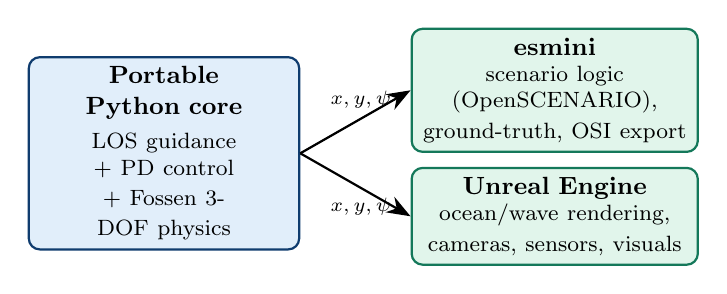
\begin{tikzpicture}[
    node distance=6mm and 14mm,
    core/.style={rectangle, rounded corners, draw=navyblue, thick, fill=lightblue,
        minimum height=22mm, text width=32mm, align=center, font=\small},
    eng/.style={rectangle, rounded corners, draw=seagreen, thick, fill=lightgreen,
        minimum height=11mm, text width=34mm, align=center, font=\small},
    arr/.style={-{Stealth[length=3mm]}, thick}
]
\node[core] (core) {\textbf{Portable Python core}\\[3pt]\footnotesize LOS guidance\\ + PD control\\ + Fossen 3-DOF physics};
\node[eng, right=of core, yshift=8mm] (esmini) {\textbf{esmini}\\\footnotesize scenario logic (OpenSCENARIO),\\ ground-truth, OSI export};
\node[eng, right=of core, yshift=-8mm] (unreal) {\textbf{Unreal Engine}\\\footnotesize ocean/wave rendering,\\ cameras, sensors, visuals};

\draw[arr] (core.east) -- node[above, font=\scriptsize, pos=0.55]{$x,y,\psi$} (esmini.west);
\draw[arr] (core.east) -- node[below, font=\scriptsize, pos=0.55]{$x,y,\psi$} (unreal.west);
\end{tikzpicture}
\end{center}

% ===========================================================================
\section{Implementation Languages: Python and C++}
% ===========================================================================
The project uses \textbf{both} languages deliberately, each where it is strongest. The guiding rule is:

\begin{center}
\fbox{\parbox{0.92\textwidth}{\centering
\textbf{If it runs every frame inside Unreal $\rightarrow$ C++.\\
If it sets up, drives, tests, or analyses the simulation from the outside $\rightarrow$ Python.}}}
\end{center}

\subsection*{Division of responsibility}
\renewcommand{\arraystretch}{1.3}
\begin{center}
\footnotesize
\begin{tabular}{p{6.6cm} p{6.6cm}}
\toprule
\textbf{Python --- outside the engine} & \textbf{C++ --- inside Unreal, per-frame runtime} \\
\midrule
Prototype and validate algorithms before committing them (as done for Fossen + LOS) & Fossen 3-DOF physics, control loop and actuation mapping \\
esmini orchestration via ctypes (scenario init, stepping, OSI) & Vessel \texttt{UCLASS} hierarchy (polymorphic vessel types) \\
Automated test harness / deterministic scenario batch loops & CPA/TCPA real-time evaluation over many targets \\
Telemetry analysis --- CSV, plots, metrics, cross-track error & COLREGs Behaviour Tree \emph{task nodes} (Rules 13/14/15) \\
AIS ingestion prototyping and offline parsing experiments & Sensor and camera capture, ocean/wave simulation \\
The ``ground-truth'' reference to regression-test the C++ against & Anything in the per-frame loop or crunching heavy data \\
\bottomrule
\end{tabular}
\end{center}

\noindent\textbf{Blueprints} act as a thin, tunable layer over the C++: exposing wave parameters,
wiring manual-override input, assembling behaviour trees from C++ task nodes, and HUD / state
visualisation.

\subsection*{The prototype-then-port workflow}
The two languages form a pipeline rather than an either/or choice:

\begin{center}
\begin{tikzpicture}[
    node distance=6mm and 9mm,
    step/.style={rectangle, rounded corners, draw=navyblue, thick, fill=lightblue,
        minimum height=13mm, text width=27mm, align=center, font=\scriptsize},
    stepc/.style={rectangle, rounded corners, draw=seagreen, thick, fill=lightgreen,
        minimum height=13mm, text width=27mm, align=center, font=\scriptsize},
    arr/.style={-{Stealth[length=3mm]}, thick}
]
\node[step] (a) {\textbf{1. Prototype}\\ in Python\\ (get it correct)};
\node[step, right=of a] (b) {\textbf{2. Validate}\\ log telemetry\\ as reference};
\node[stepc, right=of b] (c) {\textbf{3. Port hot path}\\ to Unreal C++\\ (make it fast)};
\node[stepc, right=of c] (d) {\textbf{4. Regression}\\ C++ vs Python\\ reference};
\draw[arr] (a) -- (b);
\draw[arr] (b) -- (c);
\draw[arr] (c) -- (d);
\draw[arr] (d.south) -- ++(0,-6mm) -| node[below, pos=0.25, font=\scriptsize]{iterate} (a.south);
\end{tikzpicture}
\end{center}

\noindent This gives Python's fast iteration for \emph{getting the algorithm right}, and C++'s efficiency
for \emph{running it in production} --- while the Python version remains a permanent correctness oracle.
Notably, the \textbf{test-automation harness stays in Python even in a C++-heavy project}, keeping
validation independent of the engine under test.

% ===========================================================================
\section{Conclusion}
% ===========================================================================
\begin{itemize}[leftmargin=1.6em]
    \item The chosen method --- \textbf{physics-driven, closed-loop Line-of-Sight guidance over a
    Fossen 3-DOF vessel model} --- is the standard approach in marine robotics and the only candidate
    that provides realistic dynamics, path-following accuracy, disturbance rejection, and a quantitative
    accuracy metric simultaneously.
    \item It is the \emph{only} option able to test the full COLREGs steering catalogue, because those
    rules are fundamentally about \emph{reactive, dynamically-realistic manoeuvring}.
    \item Its clean separation of ``brain'' (physics/control) from ``renderer'' (esmini / Unreal)
    makes it directly portable to the internship's dual-engine target.
    \item The \textbf{language split is deliberate}: Python for prototyping, orchestration, test
    automation and analysis; C++ for the per-frame Unreal runtime (physics, CPA/TCPA, sensors,
    vessel class hierarchy), with Blueprints as a thin tunable layer. The Python prototype doubles as
    the correctness reference for the C++ port.
    \item \textbf{Future work:} upgrade the controller to Model Predictive Control (MPC) for constraint-aware
    collision avoidance, and add multi-vessel target agents to exercise the give-way / stand-on rules.
\end{itemize}

\end{document}
